\documentclass[a4paper,11pt]{report}
\usepackage[italian]{babel}
\usepackage[utf8]{inputenc}
\usepackage[total={170mm,267mm},top=15mm,bottom=15mm,left=21mm,right=21mm]{geometry}
\usepackage{graphicx}
\usepackage{subcaption}
\usepackage{float}
\usepackage{hyperref}
\begin{document}

\begin{titlepage}
  \clearpage\thispagestyle{empty}
  \centering
  \vspace{1cm}
  {\normalsize Informatica - Area scientifica \\  Dipartimento di Scienze matematiche, informatiche e multimediali\\  Università di Udine \par}
  \vspace{3cm}
  {\Huge \textbf{Progetto di Social Computing \newline
  } \LARGE{Crowdsorcing con Crowd Frame  parte 1}
  }

  \vspace{4cm}
  {\Large  Parata Loris (144338) \\ Arzon Francesco (142439)\\ Dal Fabbro Lorenzo (142300)\\ }
  \vspace{12cm}
  {\normalsize Anno accademico 2020/2021}
  \pagebreak
\end{titlepage}

\tableofcontents{}
\pagebreak
\chapter{Crowd Frame}
\section{Introduzione}
Questo secondo progetto di Social Computing si suddivide in due parti, la fase di progettazione di un task di crowdsourcing e la fase di raccolta dati e analisi dei dati ottenuti da un piccolo gruppo di workers.
In questa relazione si documenta  la prima parte dell'esperimento di crowdsourcing, la progettazione del task richiesto dalla traccia.


\section{Progettazione del task}

\subsection{Obiettivo del task}
La traccia richiede di creare sei HIT differenti riguardanti tre libri, per ognuno dei quali si devono individuare tre edizioni differenti. Ogni HIT contiene tre edizioni, una per ogni libro di riferimento, per le quali ogni worker deve rispondere a 6 dimensioni differenti, quattro imposte dalla traccia e due scelte dal gruppo di progetto.
Per verificare un'eventuale preferenza di alcune tipologie di formato dei libri , abbiamo deciso di selezionare delle edizioni differenti, ma selezionandone una in formato Paperback, una in formato HardCover ed una in formato Kindle/Ebook.
\subsubsection{Lingua del task}
Abbiamo deciso di sviluppare l'intero progetto in lingua inglese, in modo da rendere il progetto il più realistico e simile ai task presenti sulla piattaforma di crowdsourcing di MTurk. Di conseguenza abbiamo scelto dei libri le cui edizioni sono scritte in lingua inglese.

\subsection{Creazione del task}
La creazione del task è stata effettuata mediante l'utilizzo dell'interfaccia grafica del framework \textbf{Crowd Frame} per la semplicità con cui si presenta la GUI. Anche se le modifiche successivamente sono state effettuate a livello di codice, vista la mancanza della possibilità di salvataggio della configurazione precedente.

\subsection{Le istruzioni inerenti al task}
Le istruzioni accolgono il worker e chiariscono l'obbiettivo del task. Chiarendo ogni eventuale dubbio sull'utilizzo dei dati raccolti e lo avvisa che non è strettamente necessario conoscere uno specifico libro o una sua specifica edizione per svolgere il task. Al worker viene indicato che è possibile rispondere alle domande anche con le sole informazioni sommarie mostrate durante il task, dando un'opinione personale riguardo al libro proposto.
\pagebreak
\subsection{Questionario}
Successivamente il worker viene sottoposto ad un insieme di questionari, composto da sette questionari standard ed una domanda CRT.
Questi quesiti ci permettono di conoscere in parte il background letterario del worker e le sue abitudini nell'acquisto di un libro.
Inoltre queste informazioni ci permettono anche di stabilire in parte la qualità delle risposte che verranno date alle dimensioni proposte.
Mentre la domanda CRT ci permette di valutare se l'utente risponde in maniera "istintiva".
\begin{itemize}
	\item How much time do you usually spend reading?
	\item How many books do you usually read during the year?
	\item What's your favorite literary genre?
	\item Do you prefer books in the original language or translated?
	\item What format do you buy most of your books in?
	\item Where do you usually find yourself reading?
	\item Based on what you choose a book to buy?
	\item A book and a pen cost \$1.10 in total. The book cost \$1.00 more than the pen. How much doest the pen cost?
\end{itemize}

\section{Il task}
\begin{figure}[H]
	\begin{subfigure}{.49\textwidth}
		\centering
		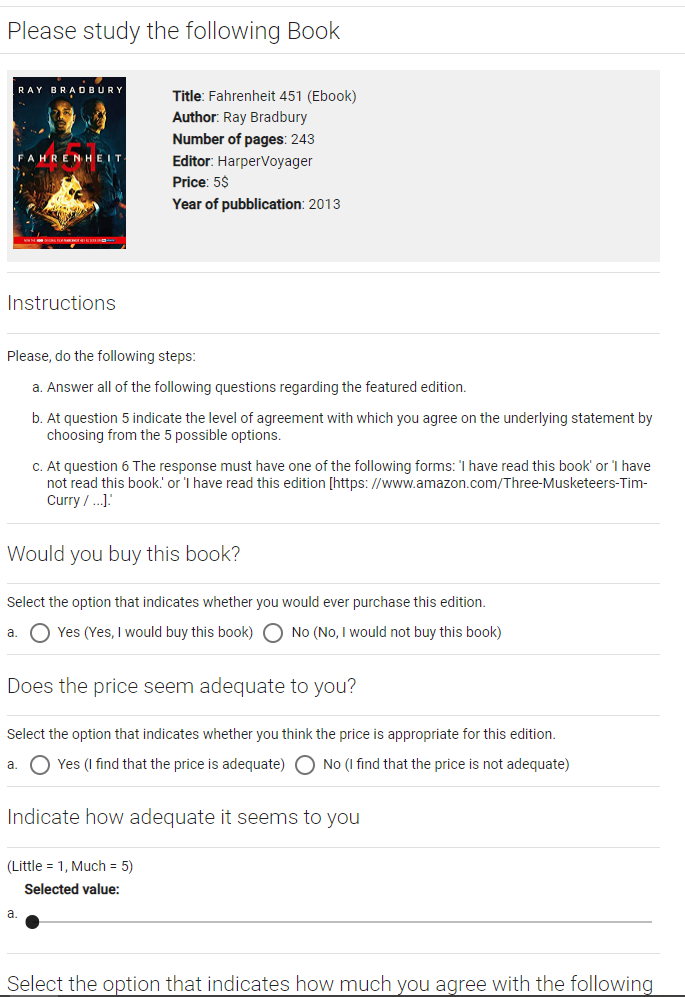
\includegraphics[width=1.043\linewidth]{task}
		\caption{Layout del task parte 1}
		\label{fig:task_layout}
	\end{subfigure}%
	\begin{subfigure}{.49\textwidth}
		\centering
		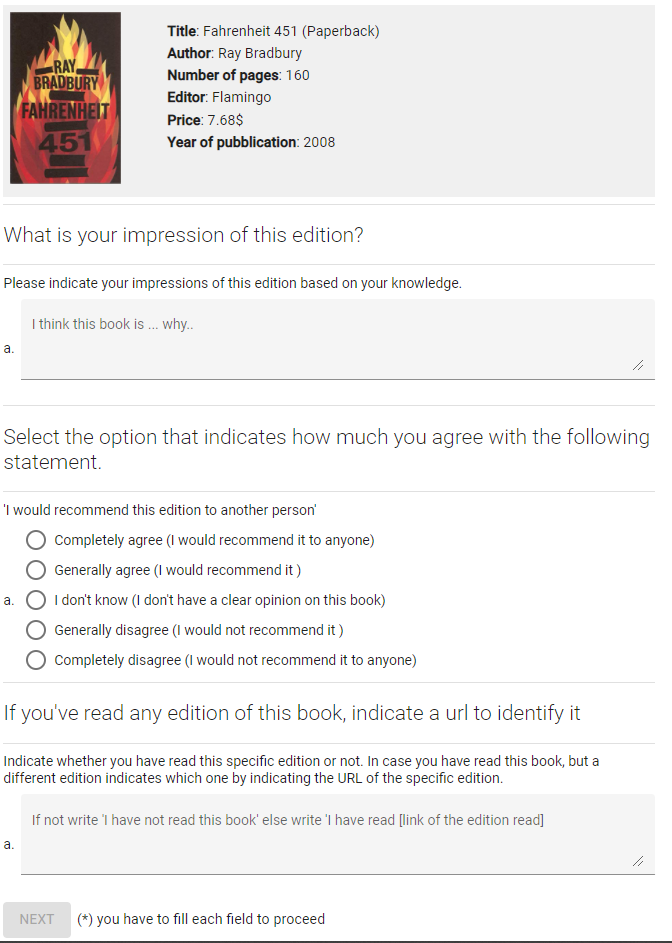
\includegraphics[width=1\linewidth]{task_p2}
		\caption{Layout del task parte 1}
		\label{fig:taskparte2}
	\end{subfigure}%
\caption{Layout del task}
\label{fig:layout}
\end{figure}
\subsection{Le dimensioni}

Ad ogni worker verranno presentate tre schermate con il layout della \textbf{Figura 1.1}
\pagebreak

Oltre alle quattro dimensioni imposte dalla traccia:
\begin{itemize}
	\item \textbf{Dimensione 1}: Would you buy this book?
	\item \textbf{Dimensione 2}: Does the price seem adequate to you?
	\item \textbf{Dimensione 3}: Indicate how adequate it seems to you
	\item \textbf{Dimensione 4}: What is your impression of this edition?
\end{itemize}
Abbiamo deciso di aggiungere :
\begin{itemize}
	\item \textbf{Dimensione 5}: Select the option that indicates how much you agree with the following statement: \\ "I would recommend this edition to another person"
	\item \textbf{Dimensione 6}: If you've read any edition of this book, indicate a URL to identify it.
\end{itemize}
\subsubsection{Dimensione 5}
La dimensione 6 è stata introdotta per verificarne la coerenza con la risposta della dimensione 1, in modo da avere un minimo di controllo ,visto il mancato utilizzo delle gold question.\\
L'utilizzo delle gold questions non è stata richiesta dalla traccia, ed essendo non ancora implementato nella GUI il controllo delle gold questions, era necessario modificare il codice del framework. La verifica di coerenza verrà effettuata nella fase di analisi.
Il worker ha a disposizione 5 possibili opzioni, che vanno dal pienamente d'accordo al completamente in disaccordo, con la possibilità di prendere una posizione neutrale relativa all'affermazione sottoposta a quesito.
\subsubsection{Dimensione 6}
La dimensione 5 è stata introdotta per verificare se il worker abbia letto una qualsiasi edizione del libro ed eventualmente individuarne delle versioni alternative preferite dai workers. Nella situazione in cui un worker non abbia mai letto quel libro si possono valutare diversamente la qualità delle risposte.   
La risposta deve essere strutturata secondo le modalità descritte nelle istruzioni del task ed un relativo controllo che richiede una risposta di almeno 4 parole. Valore individuato per scrivere la frase minima "I have read it", come scritto nelle opzioni possibili nelle istruzioni.

\subsection{Variazione del file HTML}
Per poter ottenere quel layout è stato necessario effettuare delle modifiche al file \textbf{skeleton.component.html} tra le righe 187 e 211 (\textbf{Figura 1.2 a}):
\begin{figure}[H]
	\begin{subfigure}{.60\textwidth}
		\centering
		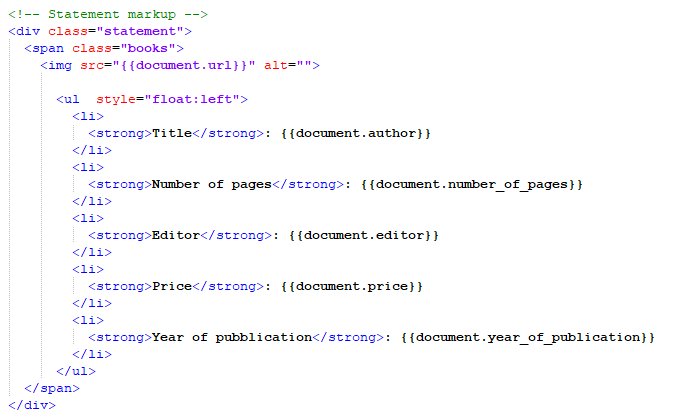
\includegraphics[width=1\linewidth]{statement}
		\caption{Codice HTML}
		\label{fig:statement}
	\end{subfigure}%
	\begin{subfigure}{.20\textwidth}
		\centering
		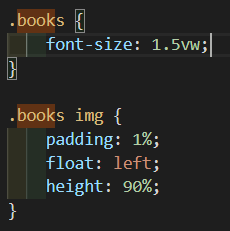
\includegraphics[width=.9\linewidth]{css}
		\caption{Classe CSS}
		\label{fig:css}
	\end{subfigure}%
	\caption{Codice HTML e CSS}
	\label{fig: HTML and CSS }
\end{figure}
In modo da visualizzare a sinistra l'immagine ed a destra gli attributi che descrivono il libro.
Le informazioni riguardanti il libro rimarranno sempre visibili al worker durante lo svolgimento del task, in modo da facilitarne lo svolgimento. \newline Inoltre è stata aggiunta una classe CSS nel file \textbf{skeleton.component.scss}, come si è può vedere in \textbf{Figura 1.2 b}, in modo da poter rendere un minimo responsive l'immagine della copertina del libro ed i relativi attributi.

\section{Struttura delle HITS}
\subsection{Generazione dei token}
Ogni HIT è accessibile ad un worker inserendo un Token che lo identifica univocamente e rilasciando nel caso di esito positivo un relativo token che permette all'utente di esser pagato dall'eventuale piattaforma di crowdsourcing.
I token e parte delle HIT sono stati generati mediante il file \textbf{hits\_tokens\_generator.ipynb}, ricevendo in input file csv contenente gli attributi che andranno a identificare ogni edizione del rispettivo libro. Adattando il codice iniziale a questo task, che ha previsto la rimozioni del codice relativo alle gold question e l'utilizzo degli attributi necessari per descrivere ogni libro. Infine verranno generati 9 oggetti contenente:
\begin{itemize}
	\item \textbf{token\_input}: token relativo alla hit che verrà assegnato al worker per accedervi.
	\item \textbf{token\_output}: token relativo alla hit che verrà assegnato al worker nel caso in cui svolge correttamente il task.
	\item \textbf{unit\_id}: per identificare la hit contenente tutti i documenti sottoposti ad esame al worker.
\end{itemize}
 E di seguito anche tutti i documenti che verranno valutati dai workers, con i relativi attributi, .
\begin{itemize}
	\item \textbf{title}: indica il titolo del libro ed il formato del libro
	\item \textbf{author}: indica l'autore/gli autori del libro o eventuali traduttori.
	\item \textbf{number of pages}: indica il numero di pagine di cui è composto il libro
	\item \textbf{editor}: indica l'editore che ha pubblicato il libro
	\item \textbf{url}: contiene l'URL che fa riferimento all'immagine della copertina del libro
	\item \textbf{year of publication}: anno di pubblicazione dell'edizione di riferimento
\end{itemize}

Di questi 9 oggetti ne verranno utilizzati 6, corrispondenti ai relativi HIT necessari. Manualmente sono stati composti i raggruppamenti dei documenti (libri) di ogni HIT. Sono stati creati 3 gruppi contenente una solo tipologia di libro (hardcover,ebook,paperback) per poter verificare eventuali preferenze nella fase di analisi. I restanti 3 sono stati creati in maniera casuale mantenendo un ordine casuale.\newline
I token generati con la relativa corrispondenza sono memorizzati nel file \textbf{data\textbackslash build\textbackslash mturk\textbackslash token.csv}

\section{Modifiche e impostazioni del task}
Nella sezione relative all'impostazione del task sono stati inseriti il nome del task e della relativa batch. Abbiamo stabilito che un worker ha a disposizione un solo tentativo ed un tempo minimo necessario a leggere un questionario o documento di \textbf{5 secondi}. Sarebbe stato ottimale poter distinguere queste due tempistiche. E' stato anche impostato un messaggio relativo alla casistica in cui un worker abbandona la sessione durante lo svolgimento e tenta di accedervi nuovamente.\newline \newline
Per accedervi al task è possibile effettuarlo accedendo alla sandbox dei worker di MTurk ed inserire la parola books nella barra di ricerca. 
Oppure direttamente accedendo tramite questo url: \url{https://parata-crowd-deploy-eu.s3.eu-central-1.amazonaws.com/Libri-task-1/Batch-libri-1/index.html}
\end{document}